\tikzset{every picture/.style={line width=0.75pt}} %set default line width to 0.75pt        

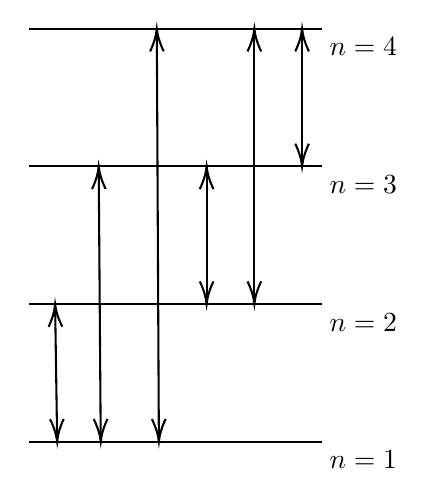
\begin{tikzpicture}[x=0.75pt,y=0.75pt,yscale=-1,xscale=1]
%uncomment if require: \path (0,425); %set diagram left start at 0, and has height of 425

%Straight Lines [id:da10159599772539862] 
\draw    (220.71,109) -- (79.29,109) ;
%Straight Lines [id:da5080837939197953] 
\draw    (220.71,175.33) -- (79.29,175.33) ;
%Straight Lines [id:da9723609878654813] 
\draw    (220.71,241.67) -- (79.29,241.67) ;
%Straight Lines [id:da4964454195724415] 
\draw    (220.71,308) -- (79.29,308) ;
%Straight Lines [id:da15757741863052366] 
\draw    (92.97,306) -- (92.03,243.67) ;
\draw [shift={(92,241.67)}, rotate = 89.14] [color={rgb, 255:red, 0; green, 0; blue, 0 }  ][line width=0.75]    (10.93,-3.29) .. controls (6.95,-1.4) and (3.31,-0.3) .. (0,0) .. controls (3.31,0.3) and (6.95,1.4) .. (10.93,3.29)   ;
\draw [shift={(93,308)}, rotate = 269.14] [color={rgb, 255:red, 0; green, 0; blue, 0 }  ][line width=0.75]    (10.93,-3.29) .. controls (6.95,-1.4) and (3.31,-0.3) .. (0,0) .. controls (3.31,0.3) and (6.95,1.4) .. (10.93,3.29)   ;
%Straight Lines [id:da399415600720878] 
\draw    (113.98,306) -- (113.02,177.33) ;
\draw [shift={(113,175.33)}, rotate = 89.57] [color={rgb, 255:red, 0; green, 0; blue, 0 }  ][line width=0.75]    (10.93,-3.29) .. controls (6.95,-1.4) and (3.31,-0.3) .. (0,0) .. controls (3.31,0.3) and (6.95,1.4) .. (10.93,3.29)   ;
\draw [shift={(114,308)}, rotate = 269.57] [color={rgb, 255:red, 0; green, 0; blue, 0 }  ][line width=0.75]    (10.93,-3.29) .. controls (6.95,-1.4) and (3.31,-0.3) .. (0,0) .. controls (3.31,0.3) and (6.95,1.4) .. (10.93,3.29)   ;
%Straight Lines [id:da39270251068842477] 
\draw    (141.99,306) -- (141.01,111) ;
\draw [shift={(141,109)}, rotate = 89.71] [color={rgb, 255:red, 0; green, 0; blue, 0 }  ][line width=0.75]    (10.93,-3.29) .. controls (6.95,-1.4) and (3.31,-0.3) .. (0,0) .. controls (3.31,0.3) and (6.95,1.4) .. (10.93,3.29)   ;
\draw [shift={(142,308)}, rotate = 269.71] [color={rgb, 255:red, 0; green, 0; blue, 0 }  ][line width=0.75]    (10.93,-3.29) .. controls (6.95,-1.4) and (3.31,-0.3) .. (0,0) .. controls (3.31,0.3) and (6.95,1.4) .. (10.93,3.29)   ;
%Straight Lines [id:da27190914055791304] 
\draw    (165,239.67) -- (165,177.33) ;
\draw [shift={(165,175.33)}, rotate = 90] [color={rgb, 255:red, 0; green, 0; blue, 0 }  ][line width=0.75]    (10.93,-3.29) .. controls (6.95,-1.4) and (3.31,-0.3) .. (0,0) .. controls (3.31,0.3) and (6.95,1.4) .. (10.93,3.29)   ;
\draw [shift={(165,241.67)}, rotate = 270] [color={rgb, 255:red, 0; green, 0; blue, 0 }  ][line width=0.75]    (10.93,-3.29) .. controls (6.95,-1.4) and (3.31,-0.3) .. (0,0) .. controls (3.31,0.3) and (6.95,1.4) .. (10.93,3.29)   ;
%Straight Lines [id:da43254530577246375] 
\draw    (188,239.67) -- (188,111) ;
\draw [shift={(188,109)}, rotate = 90] [color={rgb, 255:red, 0; green, 0; blue, 0 }  ][line width=0.75]    (10.93,-3.29) .. controls (6.95,-1.4) and (3.31,-0.3) .. (0,0) .. controls (3.31,0.3) and (6.95,1.4) .. (10.93,3.29)   ;
\draw [shift={(188,241.67)}, rotate = 270] [color={rgb, 255:red, 0; green, 0; blue, 0 }  ][line width=0.75]    (10.93,-3.29) .. controls (6.95,-1.4) and (3.31,-0.3) .. (0,0) .. controls (3.31,0.3) and (6.95,1.4) .. (10.93,3.29)   ;
%Straight Lines [id:da2755208448822286] 
\draw    (211,173.33) -- (211,111) ;
\draw [shift={(211,109)}, rotate = 90] [color={rgb, 255:red, 0; green, 0; blue, 0 }  ][line width=0.75]    (10.93,-3.29) .. controls (6.95,-1.4) and (3.31,-0.3) .. (0,0) .. controls (3.31,0.3) and (6.95,1.4) .. (10.93,3.29)   ;
\draw [shift={(211,175.33)}, rotate = 270] [color={rgb, 255:red, 0; green, 0; blue, 0 }  ][line width=0.75]    (10.93,-3.29) .. controls (6.95,-1.4) and (3.31,-0.3) .. (0,0) .. controls (3.31,0.3) and (6.95,1.4) .. (10.93,3.29)   ;

% Text Node
\draw (222.71,311) node [anchor=north west][inner sep=0.75pt]   [align=left] {$\displaystyle n=1$};
% Text Node
\draw (222.71,244.67) node [anchor=north west][inner sep=0.75pt]   [align=left] {$\displaystyle n=2$};
% Text Node
\draw (222.71,178.33) node [anchor=north west][inner sep=0.75pt]   [align=left] {$\displaystyle n=3$};
% Text Node
\draw (222.71,112) node [anchor=north west][inner sep=0.75pt]   [align=left] {$\displaystyle n=4$};


\end{tikzpicture}
